\chapter{Literature Review}\label{chap:literature_review}
This chapter reviews the literature on MTMCT and discusses the trends, advances and milestones in the field. It will focus only on the most recent and state-of-the-art methods and technologies and will not cover the entire history of MTMCT, including all past algorithms and methods. The chapter is structured as follows: Section~\ref{sec:the_beginnings} discusses the beginnings of MTMCT, Section~\ref{sec:milestones} highlights the milestones, Section~\ref{sec:methods} reviews the methods and algorithms used in MTMCT.

\section{The Beginnings}\label{sec:the_beginnings}
Back in \citeyear{Cai99} and \citeyear{Chang01}, \textcite{Cai99} and \textcite{Chang01} did research on tracking people in a multi-camera system. Also in \citeyear{Khan01}, \textcite{Khan01} proposed a method for tracking people and vehicles with uncalibrated cameras. The system is able to discover spatial relationships between the FOVs of the three cameras used. All three works rely on Bayesian classification and networks~\cite{Pearl88}.

These methods have even demonstrated the feasibility of tracking people in real-time, but are generally very limited in their capabilities. For example, the work of \citeauthor{Chang01} is limited to people in an upright pose. The algorithm proposed by \citeauthor{Cai99} lacks robustness compared to single-camera tracking and the approach of \citeauthor{Khan01} does not properly calibrate the cameras and is highly susceptible to errors caused by occlusion. In the last two decades, however, the field of multi-camera tracking has evolved significantly.

\section{Milestones}\label{sec:milestones}
This section highlights significant milestones that have shaped the field of MTMCT research, focusing on five critical areas: detection, feature extraction, data association, tracking, and datasets and challenges.

\begin{figure}[ht]
	\centering
	\begin{tikzpicture}[node distance=1cm and 4cm, auto]
	% Milestones
	\node (m1) [milestone] {Detection};
	\node (m2) [milestone, below=of m1] {Feature Extraction};
	\node (m3) [milestone, below=of m2] {Data Association};
	\node (m4) [milestone, below=of m3] {Tracking};
	\node (m5) [milestone, below=of m4] {Datasets and Challenges};

	% Techniques
	\node (t1) [technique, right=of m1] {(Faster) R-CNN, YOLO, SSD};
	\node (t2) [technique, right=of m2, below=of t1] {SIFT, HOG, CNNs};
	\node (t3) [technique, right=of m3, below=of t2] {Hungarian Algorithm, JPDAF, POM, RNNs};
	\node (t4) [technique, right=of m4, below=of t3] {Kalman Filter, MHT};
	\node (t5) [technique, right=of m5, below=of t4] {see Table~\ref{tab:overview_datasets}};

	% Arrows
	\draw [arrow] (m1) -- (m2);
	\draw [arrow] (m2) -- (m3);
	\draw [arrow] (m3) -- (m4);
	\draw [arrow] (m4) -- (m5);

	% Connections
	\draw [arrow] (t1) -- (m1);
	\draw [arrow] (t2) -- (m2);
	\draw [arrow] (t3) -- (m3);
	\draw [arrow] (t4) -- (m4);
	\draw [arrow] (t5) -- (m5);
\end{tikzpicture}
	\caption{Milestones in MTMCT}\label{fig:milestones}
\end{figure}

The Figure~\ref{fig:milestones} shows the algorithms and techniques in the green boxes (right) that correspond to each milestone area in the blue box (left). The following subsections discuss the techniques in more detail.

\subsection{Detection}\label{subsec:milestone_detection}
The foundation for modern object detection methods was laid in \citeyear{Lecun98} by \citeauthor{Lecun98} with the development of Convolutional Neural Networks (CNNs), which are deep learning models designed specifically for image processing~\cite{Lecun98}. The advent of deep learning in the last quarter century has led to a significant improvement in object detection performance.

With the introduction of R-CNN~\cite{Girshick14} in \citeyear{Girshick14}, \citeauthor{Girshick14} demonstrated that deep learning can be used for object detection. The architecture follows a two-stage process: first, it proposes Regions of Interest (RoI) using selective search and then classifies these regions using CNN features. Because R-CNN proposed RoI independently, it was computationally expensive. Just a year later, improvements were made with Fast R-CNN~\cite{Girshick15}, which addressed the inefficiencies of its predecessor by introducing a mechanism to share convolutional computations across region proposals and by incorporating a RoI pooling layer to extract a fixed-size feature vector from the feature map for each proposal. In \citeyear{Ren17} \citeauthor{Ren17} proposed Faster R-CNN~\cite{Ren17}, which integrates a Region Proposal Network (RPN) into the architecture that uses anchors, which are predefined reference boxes of various scales and aspect ratios, as the basis for proposing potential object locations. This allows the generation of region proposals at almost no cost by sharing the convolutional features with the downstream detection network. This end-to-end trainable model marked a significant leap in efficiency and set a new standard for object detection tasks.

Following the success of R-CNN and its successors, the object detection landscape was further revolutionized by the introduction of You-Only-Look-Once (YOLO)~\cite{Redmon15} and Single Shot MultiBox Detector (SSD)~\cite{Liu16}, which were designed to be even more efficient and suitable for real-time applications.

The YOLO framework, introduced by \citeauthor{Redmon15} in \citeyear{Redmon15}, revolutionized real-time object detection by predicting bounding boxes and class probabilities directly from full images in a single evaluation. YOLO processes the entire image in a single forward pass through the network, divides the image into a grid, and predicts bounding boxes and probabilities for each grid cell. The strength of YOLO lies in its speed, which makes it very suitable for applications where real-time detection is critical. Although the original author has stopped working on YOLO due to ethical concerns, it is still being improved. The latest official version, YOLOv4~\cite{Bochkovskiy20}, was released in \citeyear{Bochkovskiy20} by \citeauthor{Bochkovskiy20}. In \citeyear{Jocher23a} Ultralytics released the most recent version YOLOv8~\cite{Jocher23a, Jocher23b}.

\citeauthor{Liu16} proposed SSD in \citeyear{Liu16}, another influential single-shot object detector that balances the tradeoff between speed and accuracy. Unlike YOLO, SSD operates on multiple feature maps at different resolutions to effectively handle objects of different sizes. The architecture applies a set of convolutional filters to these feature maps to predict both bounding box offsets and class probabilities for a fixed set of default bounding boxes distributed across the image. The ability to detect and track objects across multiple scales and perspectives makes SSD particularly well-suited for MTMCT applications.

\begin{table}[ht]
	\centering
	\caption{Overview Object Detectors}\label{tab:overview_object_detectors}
	\resizebox{\textwidth}{!}{
		\begin{tabular}{|l|c|c|c|}
			\hline
			\textbf{Model}            & \textbf{Speed} & \textbf{Accuracy} & \textbf{Computational Requirements} \\
			\hline
			Faster R-CNN~\cite{Ren17} & Moderate       & High              & High                                \\
			YOLO~\cite{Redmon15}      & Very High      & Moderate          & Low                                 \\
			SSD~\cite{Liu16}          & High           & High              & Moderate                            \\
			\hline
		\end{tabular}
	}
\end{table}

The Table~\ref{tab:overview_object_detectors} compares the mentioned prominent object detection models used in MTMCT:

\begin{itemize}
	\item \textbf{Speed:} Refers to the time it takes the detector to process a single frame, usually measured in milliseconds. High speed is critical for real-time tracking applications where live or near-live video feeds must be processed.
	\item \textbf{Accuracy:} Measures the ability to correctly identify and locate objects. It is usually quantified in terms of precision and recall rates, or average precision (AP) over a dataset.
	\item \textbf{Computational Requirements:} Refers to the resources required to run the detector, typically measured in terms of floating-point operations (FLOPs) or memory and processing power. Efficient use of computational resources is essential for deploying MTMCT systems on hardware with limited capabilities.
\end{itemize}

\subsection{Feature Extraction}\label{subsec:milestone:eature_extraction}
Early feature extraction techniques relied on hand-crafted descriptors such as Scale-Invariant Feature Transform (SIFT)~\cite{Lowe04} and Histogram of Oriented Gradients (HOG)~\cite{Dalal05}, which were crucial for object recognition and re-ID tasks. With the introduction of deep learning, CNNs have enabled automatic learning of feature representations, greatly improving robustness and power for re-ID~\cite{Krizhevsky12, He16}.

More recently, Siamese networks have emerged as a popular choice for learning discriminative features in a pairwise fashion, proving highly effective for re-ID tasks~\cite{Varior16}.

\subsection{Data Association}\label{subsec:milestone_data_association}
Data association in MTMCT involves matching detections of the same object across different frames and camera views, which is essential for maintaining object ID over time. The Hungarian Algorithm~\cite{Kuhn55}, also known as the Munkres assignment algorithm, has historically been used for optimal assignment in data association, addressing the problem of associating detections to trajectories in a globally optimal way.

The complexity of data association increased with the need to handle multiple objects and cameras, leading to the development of Joint Probabilistic Data Association Filters (JPDAF)~\cite{Fortmann83}, which consider the probabilities of all potential measurement-to-track assignments.

\citeauthor{Fleuret08} introduced the use of Probabilistic Occupancy Map (POM)~\cite{Fleuret08} to model targets in a POM and combine occupancy probabilities with color and motion attributes in the tracking process in \citeyear{Fleuret08}. The POM is a ground plane that represents the occupancy probability of each cell, with this approach it is possible to track multiple people in a complex environment. The POM is still used in recent and state-of-the-art approaches.

The advent of graph-based approaches provided a robust framework for data association by viewing the problem as finding the shortest path in a graph, where each node represents a detection and edges represent association costs~\cite{Zhang08}. This method became particularly useful for managing associations over long-time periods and occlusions.

More recently, with the rise of deep learning, \textcite{Milan16b} use Recurrent Neural Networks (RNNs)~\cite{Rumelhart86} to learn the data association task, enabling an end-to-end approach to online multi-target tracking.

\subsection{Tracking}\label{subsec:milestone_tracking}
The Kalman Filter~\cite{Kalman60} is one of the early foundations of object tracking, providing a framework for predicting the future locations of an object.

As tracking scenarios became more complex, approaches such as Multiple Hypothesis Tracking (MHT)~\cite{Blackman04} were developed to manage multiple potential data association hypotheses, especially in cluttered scenes~\cite{Reid79}.

\subsection{Datasets and Challenges}\label{subsec:datasets_and_challenges}
In addition to the datasets mentioned in the Section~\ref{sec:datasets}, which are used for object detection in general, there are also datasets that are more specific to MTMCT. Typically, these are for tracking specific object classes, mainly people and vehicles. Datasets that meet these requirements are listed in the Table~\ref{tab:overview_datasets}.

\begin{table}[ht]
	\centering
	\caption{Overview of Datasets}\label{tab:overview_datasets}
	\resizebox{\textwidth}{!}{
		\begin{tabular}{|l|c|c|c|c|c|c|c|c|}
			\hline
			\textbf{Dataset}                     & \textbf{Environment} & \textbf{Num. of Scenarios} & \textbf{Num. of Cameras (Overlap)} & \textbf{FPS} & \textbf{IDs} & \textbf{Year} & \textbf{Class}  \\
			\hline
			PETS~\cite{Ferryman09}               & Outdoor              & 3                          & 8 (\cmark)                         & 25           & ---          & 2009          & Person          \\
			MARS\footnotemark[1]~\cite{Zheng16b} & Mixed                & Multiple                   & 6 (\cmark)                         & ---          & 1261         & 2016          & Person          \\
			MOT16~\cite{Milan16a}                & Outdoor              & 14                         & 1                                  & 25-30        & ---          & 2016          & Person, Vehicle \\
			DukeMTMC~\cite{Ristani16}            & Outdoor              & 1                          & 8 (\cmark)                         & 60           & 2834         & 2016          & Person          \\
			MOT17~\cite{Milan16a}                & Outdoor              & 14                         & 1                                  & 25-30        & ---          & 2018          & Person          \\
			Wildtrack~\cite{Chavdarova18}        & Outdoor              & Multiple                   & 7 (\cmark)                         & 2            & 313          & 2018          & Person          \\
			MSMT17~\cite{Wei18}                  & Mixed                & 12                         & 15 (\cmark)                        & 15           & 4101         & 2018          & Person          \\
			CityFlowV1~\cite{Tang19}             & Outdoor              & 5                          & 40 (\cmark)                        & 10           & 666          & 2019          & Vehicle         \\
			MOT20~\cite{Dendorfer20}             & Outdoor              & 8                          & 1                                  & 25           & ---          & 2020          & Person, Vehicle \\
			CityFlowV2~\cite{Tang19}             & Outdoor              & 6                          & 46 (\cmark)                        & 10           & 880          & 2021          & Vehicle         \\
			MMPTRACK~\cite{Han23}                & Indoor               & 5                          & 23 (\cmark)                        & 15           & ---          & 2023          & Person          \\
			MEVID~\cite{Davila23}                & Mixed                & 17                         & 33 (\cmark)                        & ---          & 158          & 2023          & Person          \\
			\hline
		\end{tabular}
	}
\end{table}
\footnotetext[1]{extension of Market-1501~\cite{Zheng15}}

The Table~\ref{tab:overview_datasets} provides a summary of various datasets that have made significant contributions to the MTMCT research field. Each dataset is categorized based on several different criteria to reflect its unique characteristics and relevance:

\begin{itemize}
	\item \textbf{Environment:} Data collection setting, from controlled indoor environments to dynamic outdoor locations.
	\item \textbf{Num. of Scenarios:} Specifies the number of distinct scenarios or situations represented in the dataset.
	\item \textbf{Num. of Cameras (Overlap):} Returns the number of cameras involved and indicates whether there is overlap in their views.
	\item \textbf{FPS:} Indicates the frame rate of the dataset, important for real-time processing considerations.
	\item \textbf{IDs:} Enumerates the unique IDs present, which can provide a measure of the complexity of the dataset.
	\item \textbf{Year:} Returns the year of publication, which represents the timeliness of the dataset.
	\item \textbf{Class:} Identifies the annotated classes, such as persons or vehicles.
\end{itemize}

Each of the datasets listed plays a role in the following sections and the literature reviewed is often evaluated using one or more of these datasets. The datasets are also used to train and test the tracking methods.

\begin{figure}[ht]
	\centering
	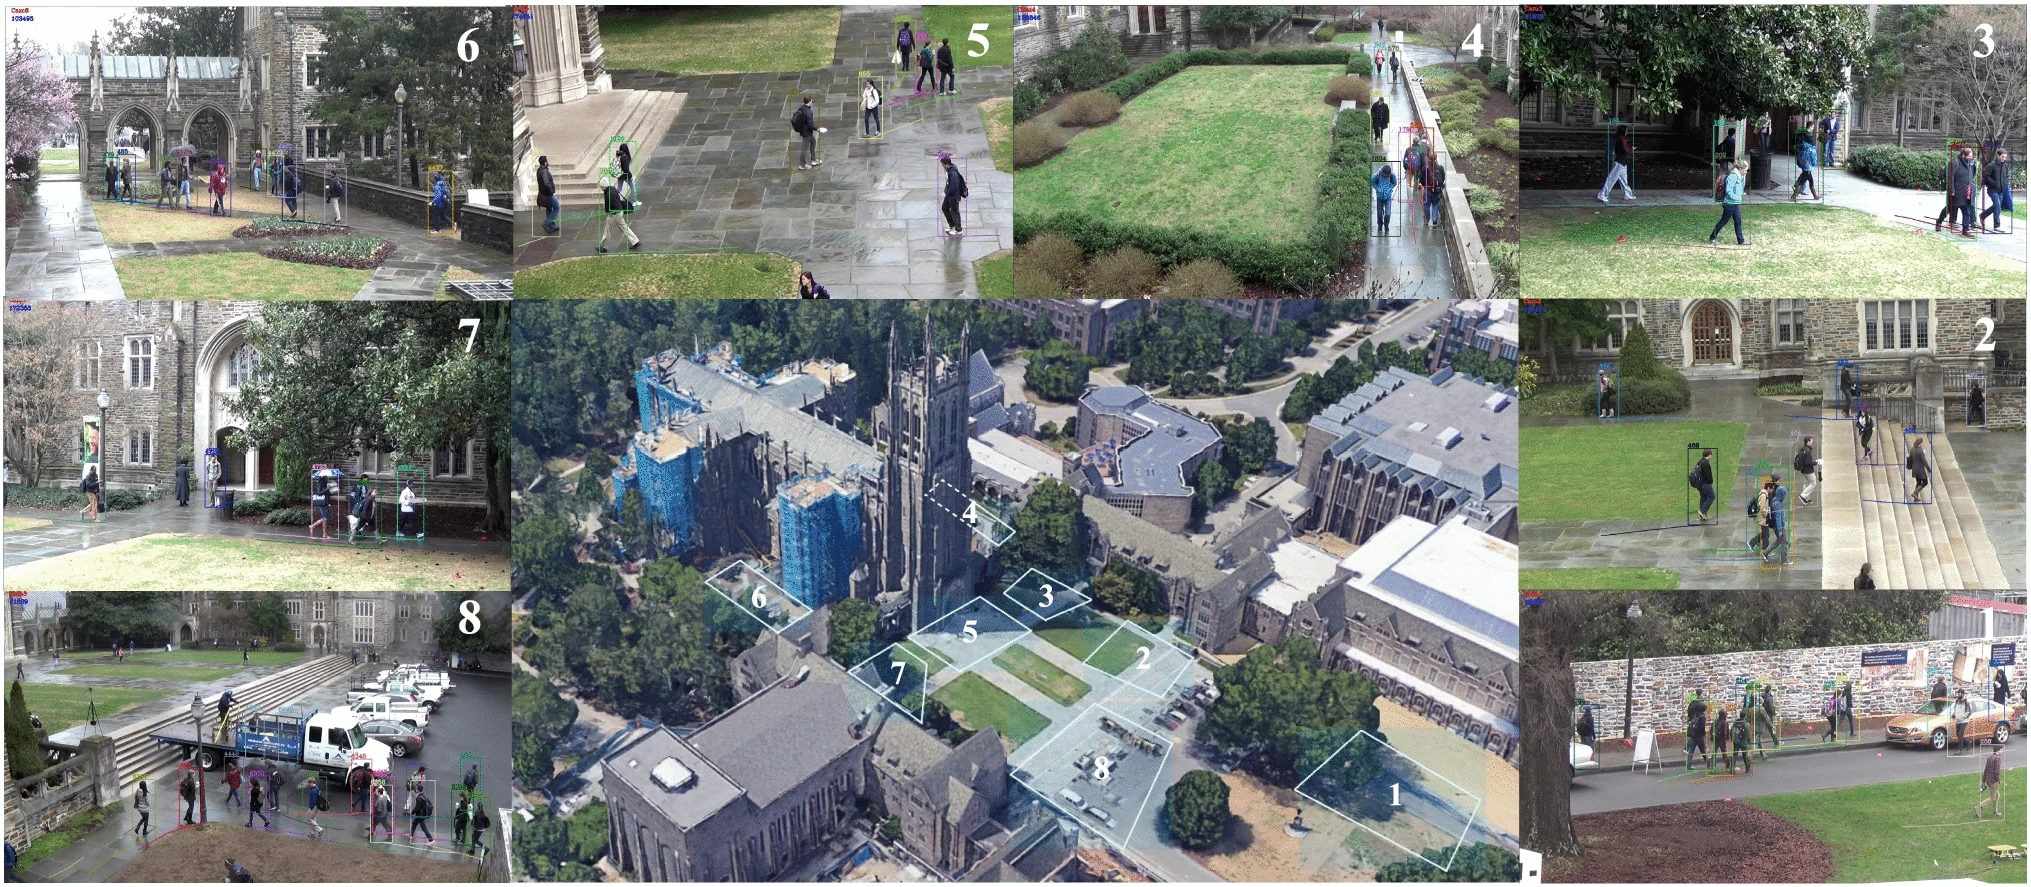
\includegraphics[width=0.75\textwidth]{resources/fig/Ma21-dukemtmc.png}
	\caption[DukeMTMC]{DukeMTMC~\cite[source image:][Fig.~2]{Ma21}}\label{fig:dukemtmc}
\end{figure}

Figure~\ref{fig:dukemtmc} visualizes part of the DukeMTMC dataset as an example of one of the MTMCT datasets. It shows the camera views of the Duke University campus used in the dataset, illustrating the variety of scenes and perspectives for tracking individuals across different locations and conditions. The central aerial view shows the spatial arrangement of the cameras, with their respective FOVs highlighted. All eight camera views are shown in a given frame, including the bounding boxes of the tracked individuals.

In recent years, challenges have been established to encourage research in object detection and tracking, although they have mostly focused on STSCT and MTSCT. Nevertheless, these challenges remain relevant to MTMCT research. The most recent representatives of the primary challenges are:

\begin{itemize}
	\item \textbf{MOT20 Challenge:} Benchmark, which includes crowded environments and variable lighting conditions. It also provides ground truth data to facilitate evaluation. The MOT datasets are released in conjunction with the MOTChallenge~\cite{Dendorfer20}.
	\item \textbf{2023 AICity Challenge:} Focuses on AI applications in smart cities and includes multi-object tracking for traffic monitoring and anomaly detection as one of its key components. The CityFlow datasets are part of the AICity Challenges~\cite{Naphade23}.
	\item \textbf{VOT2022 Challenge (Visual Object Tracking Challenge):} An annual competition that provides a standardized dataset and evaluation framework for tracking single objects~\cite{Kristan22}.
	\item \textbf{VOTS2023 Challenge (Visual Object Tracking and Segmentation Challenge):} An extension of the VOT Challenge that focuses on multi-object tracking. Recently published in October 2023, the challenge confirms the rapidly growing interest in this area~\cite{Kristan23}.
\end{itemize}

\section{Methods}\label{sec:methods}
This section reviews the methods and state-of-the-art algorithms used in MTMCT.

\subsection{Tracking Paradigms}\label{subsec:tracking_paradigms}
In recent years, several tracking paradigms have been developed and used in MTMCT. The most common paradigms are tracking-by-detection, tracking-by-regression, tracking-by-segmentation, and tracking-by-attention. Each of these paradigms has its own advantages and disadvantages, which are discussed in the following sections.

\subsubsection{Tracking-by-Detection}\label{subsubsec:tracking-by-detection}
The most common approach used by MTMCT systems is to first detect the objects in each frame and then perform data association to link the detections across frames. This Tracking-by-Detection (TbD) implementation is a multi-shot approach that treats detection and association as separate, sequential tasks, allowing the use of specialized methods tailored for each step.

\citeauthor{Bewley16} proposed one of the pioneering works in this area, the Simple Online and Realtime Tracking (SORT)~\cite{Bewley16} algorithm. SORT uses a combination of Kalman Filters to predict the motion of objects and the Hungarian Algorithm to associate detections over time based on both predicted locations and detected bounding boxes. Its efficiency and speed make it suitable for real-time applications, although it may struggle with ID switches in crowded scenes due to its reliance on motion cues alone.

Building on the foundation laid by SORT, the DeepSORT~\cite{Wojke17} algorithm was introduced by \citeauthor{Wojke17}, which improves tracking performance by incorporating deep learning techniques for extracting of appearance features. DeepSORT extends SORT by adding a neural network that generates a high-dimensional vector representation of the appearance of an object, which can be used to compute similarity scores between detections. This addition significantly improves the robustness of the tracker in scenarios where motion prediction is insufficient, such as occlusions or complex, dynamic environments.

Both SORT and DeepSORT have set benchmarks in object tracking, demonstrating how the integration of motion and appearance information can lead to improved tracking performance.

\begin{itemize}
	\item \textbf{SORT:} Focuses on speed and simplicity by using motion models for prediction and frame-by-frame data association.
	\item \textbf{DeepSORT:} Enhances SORT by adding appearance information to the data association step, improving tracking accuracy, especially in cases where objects interact closely or are temporarily occluded.
\end{itemize}

It is important to note that both tracking frameworks rely on an external object detector to provide bounding box detections, which can be any of the object detection models discussed in the Section~\ref{subsec:milestone_detection}. Neither SORT nor DeepSORT can perform inter-camera tracking; this step must be performed separately.

\subsubsection{Tracking-by-Regression}\label{subsubsec:tracking-by-regression}
Tracking-by-Regression (TbR) involves directly estimating the position of the object in each frame of a video sequence. In contrast to the TbD approach, regression-based methods predict changes in position of the object. Most approaches learn a regression function from the input image features to the position coordinates. The advantage of this method is its ability to continuously refine the estimated position, making it well-suited for scenarios with smooth motion or predictable trajectory patterns.

\subsubsection{Tracking-by-Segmentation}\label{subsubsec:tracking-by-segmentation}
Tracking-by-Segmentation (TbS), on the other hand, focuses on delineating the precise shape of the target object in each frame. This method not only tracks the position of the object, but also provides its detailed segmentation, capturing its exact outline and shape. It is particularly useful in complex scenes where the object may change shape, size, or orientation. By combining tracking and segmentation, this approach provides more detailed and accurate object tracking, especially in environments where distinguishing between foreground and background is critical.

\subsubsection{Tracking-by-Attention}\label{subsubsec:tracking_by_attention}Tracking-by-Attention (TbA) represents a paradigm shift in MTMCT systems by incorporating attention mechanisms that prioritize the most salient features of objects during tracking. The attention paradigm, inspired by the visual ability of humans to selectively focus, has been integrated into tracking frameworks to dynamically highlight important spatial and temporal features.

\subsection{Single-Shot Approaches}\label{subsec:single-shot_approaches}
In contrast to all of the above tracking paradigms, single-shot approaches aim to perform detection and data association simultaneously in a single-step. While less common, this approach offers the advantage of speed and simplicity by eliminating the need for separate data association algorithms. Especially in scenarios where computational resources are limited and real-time performance is critical, single-shot approaches can be very effective.

A notable contribution in this area is the Single-Shot Multi Object Tracking (SMOT)~\cite{Li20} algorithm proposed by \citeauthor{Li20} in \citeyear{Li20}. SMOT is a tracking framework capable of converting any single-shot object detector into a multi-object tracker, which is able to simultaneously generate detection and tracking outputs. It is based on the work of \citeauthor{Bergmann19}, who developed the Tracktor~\cite{Bergmann19}, an object detector that is also able to track objects at the same time. The SMOT framework is able to generate tracklets with an almost constant runtime with respect to the number of targets, due to the use of a lightweight linking algorithm for online tracklet linking.

In the same year, \citeauthor{Wang20a} published the paper \citetitle{Wang20a}~\cite{Wang20a}, which proposes a single deep network that Jointly learns the Detection and Embedding (JDE) model. By reducing the computational cost, the system is able to achieve (near) real-time performance while being nearly as accurate as the models trained separately for detection and embedding. The architecture is based on the Feature Pyramid Network (FPN)~\cite{Lin17}, which is useful for detecting objects of different sizes. A variation of the triplet loss~\cite{Schroff15} is used to learn the embedding space, which is used for data association. This variation of the triplet loss is defined as follows:

\begin{equation}
	\label{eq:triplet_loss}
	\mathcal{L}_{\text{triplet}}=\sum_i \max \left(0, f^{\top} f_i^{-}-f^{\top} f^{+}\right)
	\quad\text{\cite[Eq.~1]{Wang20a}}
\end{equation}

\begin{itemize}
	\item \(f^{\top}\): Instance in a mini-batch selected as the anchor
	\item \(f^{+}\): Represents a positive instance (same ID as anchor)
	\item \(f^{-}\): Represents a negative instance (different ID than anchor)
\end{itemize}

The triplet loss defined in the Equation~\ref{eq:triplet_loss} is used to learn an embedding space in which instances of the same ID are closely mapped to each other, while the embeddings of different IDs are pushed apart.

A more recent framework is the FairMOT~\cite{Zhang21} algorithm proposed by \citeauthor{Zhang21} in \citeyear{Zhang21}. It combines the two tasks of object detection and re-ID, while addressing the \textit{unfairness} issue in multitask learning, which arises because re-ID is often treated as a secondary task in existing frameworks and not given enough attention. The paper raises three key issues with existing multitask learning frameworks:

\begin{enumerate}
	\item \textbf{Unfairness Caused by Anchors:} The re-ID task is overlooked in the anchor-based detection framework, where anchors are optimized only for the detection task.
	\item \textbf{Unfairness Caused by Features:} One-shot trackers share most of their features between the detection and re-ID branches. While detection requires deep features to estimate the object class, re-ID requires low-level appearance features to distinguish between different IDs, leading to a conflict between the two tasks.
	\item \textbf{Unfairness Caused by Feature Dimension:} The feature dimension of re-ID features is usually much higher than that of detection features, but high-dimensional features significantly degrade detection performance.
\end{enumerate}

To jointly train the detection and re-ID branches in the FairMOT network, the uncertainty loss proposed by \textcite{Cipolla18} is used. The uncertainty loss is defined as:

\begin{equation}
	\label{eq:uncertainty_loss}
	L_{\text{total}}=\frac{1}{2}\left(\frac{1}{e^{w_1}} L_{\text{detection}}+\frac{1}{e^{w_2}} L_{\text{identity}}+w_1+w_2\right)
	\quad\text{\cite[Eq.~5]{Zhang21}}
\end{equation}

The uncertainty loss defined in the Equation~\ref{eq:uncertainty_loss} is used to jointly train the detection and re-ID tasks by assigning different weights to the two tasks to allow for a fair learning process. The weights \(w_1\) and \(w_2\) are used to control the balance between the two tasks and are learned during training. \(L_{\text{detection}}\) and \(L_{\text{identity}}\) are the detection and re-ID losses respectively.

By addressing the three key issues with existing multitask learning frameworks, the FairMOT framework is able to outperform state-of-the-art methods in both tracking accuracy and speed on the MOT17 dataset.

An important note is that the term \textit{single-shot} used by these frameworks only refers to the detection and intra-camera tracking, the inter-camera associations still require an additional separate step.

\subsection{Graph Based Approaches}\label{subsec:graph_based_approaches}
Graph-based approaches have been widely used in MTMCT, especially for data association. The data association problem can be formulated as a graph optimization problem, where each node represents a detection and the edges represent the association costs~\cite{Zhang08}. The goal is to find the shortest path in the graph representing the sequence of object detections over time. More recently, Graph Neural Networks (GNNs)~\cite{Scarselli09} have been used to learn the data association task, allowing for an end-to-end approach to tracking.

In \citeyear{Chen17a}, \textcite{Chen17a} proposed a pedestrian tracking model that combines inter- and intra-camera tracking and unifies the two steps into a global graph by considering the initial observations as inputs and directly outputting the final trajectories. Since the initial observations contain more information such as motion than simple detections, they are more credible for data association. Furthermore, it speeds up the computation time because the number of observations is much smaller than the number of detections. The main focus of this paper is to equalize the similarity metrics of both tasks to allow unbiased data association. An equalization of the metrics is necessary because, if it is not applied, the joint approach would almost always favor objects from the same camera view as more similar because the observations are made under the same circumstances such as viewing angle and illumination. Experimental results show that the proposed joint approach leads to improved performance compared to tackling the association as two independent tasks, especially when the accuracy of intra-camera tracking quality is poor the two-step approach is not able to recover in the second step and produces mismatches errors.

Similar to~\cite{Chen17a}, \citeauthor{Nguyen22b} present a single-stage approach that combines intra- and inter-camera association by reformulating it as a single-global one-to-many assignment problem. With a focus on dynamic (on-the-move) cameras, the method is used in an autonomous vehicle (AV) environment, which is not the focus of this project, but still an interesting concept and worth mentioning. The proposed method is called Fractional Optimal Transport Assignment (FOTA)~\cite{Nguyen22b} and can be used in both TbD and TbA paradigms. The architecture consists of an encoder, two decoders and a box-matching layer. The encoder extracts features of the current and previous frames from the cameras and encodes the feature maps into keys that are used by the decoders to detect and track object boxes. The box-matching layer is then used to match the boxes and provide the final tracking results. The FOTA method results in a reduction of ID switch errors in a large AV dataset compared to state-of-the-art methods.

The Dynamic Graph Model with Link Prediction (DyGLIP)~\cite{Quach21} approach proposed by \citeauthor{Quach21} in \citeyear{Quach21} is a graph model that uses link prediction to solve the data association problem. It works for both overlapping and non-overlapping cameras and is tested on both person and vehicle tracking. The main advantages are better feature representation and the ability to recover lost tracklets during camera transitions. DyGLIP combines link prediction with a dynamic graph formulation that, for the first time in MTMCT, takes into account temporal information of an object. Based on this approach, \citeauthor{Cheng23} propose a Reconfigurable Spatial-Temporal Graph Model (ReST)~\cite{Cheng23} in \citeyear{Cheng23}, which handles data association in two steps. First, spatial association matches objects across different views at the same frames. Before the second step, a graph reconfiguration module simplifies and reconfigures the graph. Then, temporal association uses information such as speed and time to build a temporal graph and match objects across different frames. Unlike traditional approaches, ReST does not rely on intra-camera tracking results because it directly matches inter-camera views in the first step. Another advantage is that two graph models can be trained separately, so there is no need to compromise between the two tasks of intra- and inter-camera data association. The ReST model achieves state-of-the-art performance on the Wildtrack dataset.

The graph-based soccer player tracker published by \textcite{Komorowski22} uses raw detection heat maps of the feet of the players directly instead of bounding boxes. The feet of the players are detected by the pre-trained detector FootAndBall~\cite{Komorowski20}, the detection heat maps of all cameras are transformed to a bird's eye view plane and stacked to form a multi-channel tensor. This results in the extraction and aggregation being performed within the tracking network itself, rather than in a separate preprocessing step as in conventional approaches, thus following the TbR paradigm. The tracking network consists of a Long Short-Term Memory-based (LSTM)~\cite{Gers02} RNN, which models the player dynamics and a GNN, which is able to learn the interaction between players. The training data is synthetically generated by the Google Research Football Environment (GRF)~\cite{Kurach19} and the final tracker is compared with a baseline approach based on a particle filter. Although the proposed tracker cannot use visual cues such as jersey numbers due to the large distance to the camera, it achieves better accuracy and a lower number of ID switches compared to the baseline approach.

\subsection{Edge Computing}\label{subsec:edge_computing}
The term \textit{edge computing} refers to the concept of processing data near the source of the data, as opposed to the traditional approach of processing data in a centralized cloud. The advantages of edge computing are low latency, reduced bandwidth and improved security because raw video data is not stored. The main drawback is the limited computational resources of the edge devices, in this case the cameras themselves.

In the paper on the single-shot approach SMOT discussed earlier, it is mentioned that replacing the components of the SMOT framework with faster versions can achieve real-time performance on less powerful machines such as edge devices.

\citeauthor{Wang23b} present a Multi-Camera Multi-Hypothesis Tracking (MC-MHT) framework integrated with a blockchain-based system, Multi-Camera TrackingChain (MCTChain)~\cite{Wang23b}. This extensible architecture distributes tracking tasks among cameras, improving scalability and security compared to centralized approaches. The architecture consists of three layers: the tracking, the blockchain and the edge network layer. In the experiment, 20 edge cameras are used and the tracking task is performed locally in each camera. Therefore, a leader election is implemented in the MCTChain framework to select the camera responsible for the package transaction. The proposed method achieves real-time performance (24-36 FPS).

Similar to MCTChain, the paper \citetitle{Nikodem20}~\cite{Nikodem20} introduces a decentralized tracking algorithm following the TbD paradigm, which performs intra-camera tracking locally on the camera and uses ISM-based wireless device-to-device communication for inter-camera tracking.

\subsection{Online and Real-Time}\label{subsec:online_and_real-time}
In addition to Subsections~\ref{subsec:single-shot_approaches} and~\ref{subsec:edge_computing}, which cover single-shot approaches and edge computing and their relevance to real-time applications, this subsection focuses on online and real-time implementations, mentioning specific methods.

Unlike most of the methods used in MTMCT, the real-time system Uni-ID~\cite{Chen22} follows a distributed concept to ensure that the communication and computing costs of each camera in the network remain nearly constant as the number of cameras increases. Therefore, smart stations are installed on the tracked roadside and connected by a wireless multi-hop network. YOLO is used for detection and DeepSORT for tracking. First, intra-camera tracking and feature extraction are performed to assign a local ID to each object. Second, the local ID, features and trajectory information of the target are sent to the neighboring node in the network. Third, the neighboring node performs inter-camera tracking to assign a global ID to the target. The system is tested with three nodes and achieves real-time performance with a relatively low-power GPU for each node.

The work of \textcite{Wang21} focuses on the conspicuous use of fisheye cameras to simulate a checkout-free store, where each person enters or exits the store by scanning a QR code that initializes and terminates the tracking process. Compared to perspective cameras, fisheye cameras can cover a larger area with a single-camera, reducing the number of cameras needed in the system. In addition, fisheye cameras are less susceptible to occlusion when mounted on a ceiling (top-view). Once a camera is calibrated, the POM of the scene can be created to determine the likelihood of a person being in a particular area and to match the trajectories of the same person across different cameras. In a scenario with five fisheye cameras and five to ten people in a scene simultaneously, the system achieves real-time performance of about ten FPS without GPU support.

\citeauthor{Tesfaye19} propose the use of Fast-Constrained Dominant Set Clustering (FCDSC)~\cite{Tesfaye19} to solve both intra- and inter-camera tracking simultaneously. The method is orders of magnitude faster than existing graph-based methods because it  considers only a sub-graph instead of the entire graph at each step. The proposed method follows a three-layer hierarchical approach. The first two layers solve intra-camera tracking and the third layer solves inter-camera tracking by merging the trajectories of the same person across camera views. The tracking algorithm runs at 18 FPS and is 2000 times faster than the CDSC~\cite{Zemene16} on which it is based.

\subsection{Attention Models and Transformers}\label{subsec:attention_models_and_transformers}
Recent advances in MTMCT have been influenced by the development of attention models and transformers~\cite{Vaswani17}, originally applied to natural language processing and designed to improve focus in neural networks. Despite their advantages, the high resource requirements, particularly in terms of processing power and memory, pose a challenge in achieving the low latency required for online and real-time MTMCT tracking applications. Nevertheless, examples of attention models and transformer implementations are at least mentioned in the context of this project.

The paper \citetitle{Carion20}~(DETR)~\cite{Carion20} published by \citeauthor{Carion20} in \citeyear{Carion20} lays the foundation for the use of transformers in object detection. It combines a transformer with a set-based global loss and demonstrates significant improvements in accuracy and efficiency. This work paved the way for subsequent transformer-based MOT models.

MOTR~\cite{Zeng21} extends the DETR framework by introducing a ``track query'' for tracking multiple objects across frames. MOTR updates track queries iteratively, proving temporal relation modeling and MOT performance. TrackFormer~\cite{Meinhardt22} presents an end-to-end trainable model that uses static object queries to initialize new tracks and autoregressive track queries for existing tracks. TransTrack~\cite{Sun20} introduces a method that simultaneously handles object detection and association. It uses the object features of the previous frame as a query for the current frame, simplifying the tracking process. Furthermore, MotionTrack~\cite{Zhang23} demonstrates the application of transformers in an autonomous driving environment with multiple sensor inputs.

The Dual Matching Attention Networks (DMAN)~\cite{Zhu19} approach consists of both spatial and temporal attention mechanisms. The first generates dual attention maps that allow the network to focus on the matching patterns of the input image pair, while the second adaptively allocates different levels of attention to different samples in the trajectory to suppress noisy observations.

In comparison to the aforementioned tracking frameworks, which solve the task of intra-camera tracking and are not able to perform inter-camera tracking. MVDeTr~\cite{Hou21} and the model of \textcite{Li21} are able to perform both tasks. MVDeTr focuses on the aggregation of content from multiple camera views. The introduction of the shadow transformer for effective multi-view data fusion is an important step in addressing occlusions and view inconsistencies in MTMCT. \cite{Li21} uses transformer-based attention mechanisms for robust person association across different camera views. This approach is instrumental in improving the re-ID component of MTMCT, focusing on the challenges posed by uncalibrated and overlapping camera setups.

\subsection{State-of-the-Art Approaches}\label{subsec:state-of-the-art_approaches}
This subsection presents state-of-the-art approaches published in \citeyear{Hsu22} and \citeyear{Teepe23}. The approaches achieve state-of-the-art performance on MTMCT datasets, but are not real-time applicable, due to the use of computationally expensive methods.

\citeauthor{Hsu22} introduce a Self-supervised Camera Link Model (SCLM)~\cite{Hsu22} that extracts both appearance and topological features from a Graph Auto-Encoder (GAE)~\cite{Kipf16} to achieve vehicle tracking in a multi-camera environment. The approach follows the TbD paradigm and advances the Traffic-Aware Single Camera Tracking (TSCT)~\cite{Hsu20} algorithm, which proposes a zone generation algorithm. After the common steps object detection and feature extraction, these are used as nodes for the GAE to build the camera link model and generate the tracking results. In addition, the intra-camera tracking results are used to generate entry and exit points by using the MeanShift~\cite{Comaniciu02} clustering algorithm. The combination of the TSCT and GAE embeddings with zone generation results in state-of-the-art performance on the CityFlow 2019 and 2020 datasets.

Lifted Multicut Meets Geometry Projections (LMGP)~\cite{Nguyen22a} proposed by \citeauthor{Nguyen22a} follows the traditional TbD paradigm, but with the use of POM for each node in the tracking graph, it integrates concepts from centralized representation methods. A pre-clustering step refines the tracklets generated by intra-camera tracking to reduce ID switch errors. For the pre-clustering step, the bottom edge center of each bounding box is projected to obtain the 3D coordinates. If the Euclidean distance between two projected ground points is less than a diameter of a person, the two detections may belong to the same person. While solving a global lifted multicut formulation, the model considers short- and long-range temporal interactions  to perform inter-camera matching. Intra-camera tracking is performed by CenterTrack~\cite{Zhou20} and embedding vectors are extracted by DG-Net~\cite{Zheng19}. LMGP achieves near perfect state-of-the-art performance on the Wildtrack dataset.

EarlyBird~\cite{Teepe23} proposes early fusion in the Bird's Eye View (BEV), i.e., detections are performed directly in the BEV to solve the spatial association of pedestrians across cameras. The approach is based on MVDeTr and brings the concept of joint detection and re-ID extraction from FairMOT to MTMCT. The input frames are augmented and fed to an encoder network, the image features are projected onto the ground plane and aggregated to obtain BEV features (in BEV space). Finally, the detections and their corresponding re-ID features are fed through a decoder network to associate the detections. The proposed approach is similar to ReST in the sense that it associates spatially on the ground plane, but it has the advantage of projecting the entire feature space onto the ground plane and associating it with the decoder network. EarlyBird shows that early fusion in the BEV space can outperform late fusion in the image space. The disadvantage is higher computational cost due to the simultaneous projection of full images from all camera views onto the ground plane. It also requires high-quality 3D annotations, which are costly and rare for real-world data.

\citeauthor{Huang23a} propose a method for non-overlapping multi-camera pedestrian tracking that solves the problem of poor long-term feature storage to correctly identify people even when significant changes in appearance occur, such as different clothing or lighting conditions. The proposed method follows the TbD paradigm and combines a state-of-the-art OC-SORT-based~\cite{Cao23} tracker with the person re-ID library Torchreid~\cite{Zhou19} for feature extraction. The feature extraction is performed as a feature averaging, taking into account only those frames where the person is not occluded and is not about to leave or enter the scene. Once a new person enters the scene and has accumulated enough features, the cosine distance between the features of the new person and the people in the area is computed and the ID is restored if the distance is below a certain threshold, this works both for matching people in the same camera and across camera views. Furthermore, a new dataset containing 40000 frames recorded by three cameras is proposed to evaluate the performance of their method. Results show that the combination of OC-SORT, the proposed long-term feature extraction and Torchreid outperforms state-of-the-art methods on the new dataset. Unfortunately, the proposed method is only tested on the new dataset and not on existing datasets, which makes it difficult to compare the performance in a broader context.

\textcite{Huang23b} win first place in the AI City Challenge 2023 (Track1) with their anchor-guided clustering approach for inter-camera re-ID, enabled by self-camera calibrations to improve the tracking accuracy of people with similar appearance. Three steps are performed to achieve the final tracking results. First, intra-camera tracking is performed with BoT-SORT~\cite{Aharon22} following a standard TbD scheme. Second, the anchor-guided clustering step fixes ID switches and assigns a global ID to each trajectory by hierarchically clustering appearance features from each camera view and obtaining anchors. Each anchor contains features that represent the appearance of the same ID under different conditions. Third, human pose with camera self-calibration is used to project the tracked objects onto a top-down map.

The \citetitle{Kristan23} presents the performance of the 47 trackers submitted to the challenge. Most of the trackers use a uniform dynamic model and transformers. Both multi- and single-shot approaches are used, but the top three trackers are single-shot approaches. The top tracker DMAOT is based on the VOT22~\cite{Kristan22} winner AOT~\cite{Yang21} and its successor DeAOT~\cite{Yang22b}. Although detailed technical documentation of DMAOT is currently unavailable, it is known to store long-term memory by object rather than by frame to predict object masks. Overall, the challenge shows a paradigm shift from bounding-box trackers to segmentation-based trackers that outperform all bounding-box trackers in the challenge.

\subsection{Honorable Mentions}\label{subsec:honorable_mentions}
In the exploration of advanced tracking methods, certain studies stand out for their unique and unconventional approaches. This subsection highlights two of these studies that are not directly related to real-time MTMCT but still deserve honorable mentions.

An interesting development in the field of people tracking is \citetitle{Yu13}~\cite{Yu13} from \citeyear{Yu13}. Drawing parallels to the fictional ``Marauder's Map'' in the Harry Potter series, this research proposes a framework that follows the TbD paradigm and uses non-negative discretization for robust localization and tracking of people in complex environments. Their method overcomes challenges such as occlusion and sparse surveillance camera coverage by employing a semi-supervised learning framework that integrates cues such as color, person detection, face recognition, and non-background information. Its application in a real-world nursing home environment, captured by 15 cameras, demonstrates its effectiveness in indoor scenarios.

Equally intriguing is the paper \citetitle{Koehl20}~\cite{Koehl20}, a unique dataset for MTMCT research captured within the virtual environment of the popular video game Grand Theft Auto V (GTA). This creative approach leverages the complex, dynamic world of GTA to provide a rich, diverse dataset for tracking research, highlighting the innovative ways in which simulated environments can contribute to the advancement of computer vision without invading the privacy of individuals.